\section{Implementierung}
\label{sec:implementation}

Nachdem das grobe Konzept der Dateiverwaltung der Schul-Cloud geschildert wurde, werden anschließend wirkliche Implementierungsdetails präsentiert. Diese wird in einer Zweiteilung erfolgen. Zunächst wird relevanter Code des Schul-Cloud Servers \footnote{Schul-Cloud Server - \url{https://github.com/schul-cloud/schulcloud-server}} aufgezeigt und beschrieben. Dann werden dazu passende Teile vom User Interfaces des Schul-Cloud Clients \footnote{Schul-Cloud Client - \url{https://github.com/schul-cloud/schulcloud-client}} dargelegt. Beide Komponenten sind öffentlich auf GitHub \footnote{GitHub - \url{https://github.com}} zugänglich.

\subsection{Schul-Cloud Server}
\subsubsection{Einbettung in das Schul-Cloud - Datenmodell}

Der Schul-Cloud Server basiert auf Node.js \footnote{Node.js - \url{https://nodejs.org}} und Feathers \footnote{Feathers - \url{https://feathersjs.com/}}, einer auf Express \footnote{Express - \url{http://expressjs.com/de/}} aufbauenden Schicht für das schnelle Entwickeln von REST-APIs \footnote{Representational State Transfer (REST) - \url{https://de.wikipedia.org/wiki/Representational_State_Transfer}}. Die Dateiverwaltung des Backends wird somit auch als typischer Feathers-Service bereitgestellt. Dieser befindet sich im Unterordner \textit{src/services/fileStorage} und beinhaltet die grundlegende Funktionalität der Dateiverwaltung. Anders als typische Feathers Services besitzt dieser kein MongoDB \footnote{MongoDB - \url{https://www.mongodb.com/de}} - Model, sondern dient eher als Proxy-Service. Die \textit{index.js} bündelt die drei Teilservices des File-Storage Services zusammen und macht sie nach außen zugänglich (Appendix \ref{code:filestorageindex}). Diese sind zum einem der \textit{FileStorageService}, welcher sich um die eigentliche Verteilung von Dateianfragen, wie das Erstellen und Löschen von Dateien, kümmert. Dazu kommt der \textit{SignedUrlService}, welcher die Zugriffslink generiert. Als drittes gibt es den \textit{DirectoryService}, welcher zusätzliche Funktionalitäten für Ordner bereit stellt. Alle API-Routen werden unter \textit{/fileStorage/} registriert, wobei der \textit{SignedUrlService} unter \textit{/fileStorage/signedUrl} und der \textit{DirectoryService} unter \textit{/fileStorage/directories} verfügbar ist. Die einzelnen Funktionen aller API-Routen sind in der Dokumentation des Servers \cite{online:serverswagger} verfügbar. \\

In der \textit{index.js} des FileStorage Services erfolgt außerdem die Auswahl der richtigen Strategie für die Schule des Zugreifenden auf die API. Eine in der Schul-Cloud vermerkte Schule kann genau einen \textit{fileStorageType} besitzen, wie die \textit{model.js} des SchoolServices (\textit{src/services/school}) des Backend zeigt:

\begin{lstlisting}[label= schoolModel]
	'use strict';

	const fileStorageTypes = ['awsS3']; // aktuell unterstützte Strategien
	
	const schoolSchema = new Schema({
		name: {type: String, required: true},
		address: {type: Object},
		fileStorageType: {type: String, enum: fileStorageTypes}, // Eigenschaft zur Auswahl der richtigen Strategie
		systems: [{type: Schema.Types.ObjectId, ref: 'system'}],
		federalState: {type: Schema.Types.ObjectId, ref: 'federalstate'},
		createdAt: {type: Date, 'default': Date.now},
		updatedAt: {type: Date, 'default': Date.now}
	}	,{
		timestamps: true
	});
\end{lstlisting}

Vor dem Aufrufen jeder Route wird die Funktion \textit{resolveStorageType} in \textit{src/services/fileStorage/hooks/index.js} ausgeführt, die dafür sorgt, dass der Typ des Schul-Buckets aus der im Nutzer referenzierten Schule erhalten wird. Die \textit{userId} wird vorher wie bei Feathers üblich aus dem Request via Authentifizierung ermittelt.

\begin{lstlisting}[label= resolveStorageType]
	const resolveStorageType = (hook) => {
		let userService = hook.app.service("users");
		
		// finde angemeldeten Nutzer
		return userService.find({query: {
				_id: hook.params.payload.userId,
				$populate: ['schoolId'] // hole referenzierte Schule
			}}).then(res => {
			
				// speichere korrekten Typ
				hook.params.payload.fileStorageType = res.data[0].schoolId.fileStorageType;
				return hook;
		});
	};
\end{lstlisting}

Aus dieser Information kann der FileStorage Service dann die richtige Strategie wählen. Hier ein Beispiel für die Funktion \textit{find}, welche auf \textit{GET /fileStorage/} registriert ist und die Dateien für einen gegebenen Pfad holt:

\begin{lstlisting}[label=findFiles]
	/**
	* @returns {Promise}
	* @param query contains the file path
	* @param payload contains fileStorageType and userId, set by middleware
	*/
	find({query, payload}) {
		return createCorrectStrategy(payload.fileStorageType).getFiles(payload.userId, query.path);
	}
\end{lstlisting}

Die Funktion \textit{createCorrectStrategy} erzeugt ein Objekt für die jeweilige Strategie, welche in \textit{src/services/fileStorage/strategies} implementiert sind:

\begin{lstlisting}
	const strategies = {
		awsS3: AWSStrategy
	};

	const createCorrectStrategy = (fileStorageType) => {
		const strategy = strategies[fileStorageType];
		if (!strategy) throw new errors.BadRequest("No file storage provided for this school");
		return new strategy();
	};
\end{lstlisting}

\subsubsection{AWS S3 - Strategy als Beispiel}

Im Schul-Cloud Server lassen sich eine Reihe von Strategien für verschiedene Typen von File Storage Providern implementieren. Diese werden im Ordner \textit{src/services/fileStorage/strategies} abgelegt. Die Klasse \textit{AbstractFileStorageStrategy} (Appendix \ref{code:strategyinterface}) gibt die zu implementierenden Funktionen vor. Die einzelnen Strategien sind somit Unterklassen dieser. In diesem Abschnitt wird die Implementierung für einen AWS S3-Adapter beschrieben. S3 dient während der Pilotphase der Schul-Cloud als Standart-Provider. Um schnell entwickeln zu können, wurde ein S3-Abbild auf dem Development-System der Schul-Cloud \footnote{Development-System - \url{https://schul.tech/}} eingestellt. Hierbei wurde \textit{minion} \footnote{minion - \url{https://github.com/minio/minio}} genutzt, einem Open Source Projekt, was Funktionen von S3 nachbildet. Die AWS S3-Strategy befindet sich in \textit{src/services/fileStorage/strategies/awsS3.js}. \\

Um Zugriff auf eine S3-Instanz zu bekommen, brauch die Strategie eine AWS-S3-Konfiguration. Das Node-Modul \textit{aws-sdk} \footnote{aws-sdk - \url{https://aws.amazon.com/de/sdk-for-node-js/}} bietet hierbei eine komplette Anbindungsmöglichkeit. Eine mögliche S3-Konfiguration könnte folgendermaßen aussehen:

\begin{lstlisting}
	
	const awsConfig =  {
		"signatureVersion": "v4",
		"s3ForcePathStyle": true,
		"sslEnabled": true,
		"accessKeyId": "password",
		"secretAccessKey": "password",
		"region": "eu-west-1",
		"endpointUrl": "https://localhost:3000"
	}
\end{lstlisting}

Mithilfe dieser Konfiguration und dem aws-sdk kann man nun Befehle an eine S3-Instanz schicken. Der AWS S3-Standard unterstützt alle der in der \textit{AbstractFileStorageStrategy} geforderten Funktionen. In Appendix \ref{code:awsS3deletefile} wird die Implementierung der Funktion \textit{deleteFile} für das Löschen einer Datei in einem S3-Bucket gezeigt. In jeder Funktion der Strategie muss zuerst die Berechtigung geprüft werden. Dies übernimmt der \textit{filePermissionHelper}, welcher im nächsten Abschnitt näher vorgestellt wird. Ein weiterer wichtiger Punkt beim Verbinden mit der S3-Instanz ist das Erstellen eines AWS S3-Verbindungsobjekts (Zeile 13). Dieser beinhaltet die vorher angelegte Konfiguration sowie die Information, mit welchem Bucket sich verbunden werden soll. Da die Architektur vorgibt, dass Buckets zu Schulen gehören, ergibt sich der Name des Buckets einfach aus \textit{"bucket-" + schoolId}. Die Funktion \textit{createAWSObject} zeigt die Generierung dieses Objekts:

\begin{lstlisting}
	const createAWSObject = (schoolId) => {
		if (!awsConfig.endpointUrl) throw new Error('AWS integration is not configured on the server');
		
		// Verbinden der Konfiguration
		var config = new aws.Config(awsConfig);
		
		// Einstellen des S3-Endpunktes
		config.endpoint = new aws.Endpoint(awsConfig.endpointUrl);
		
		// Einstellen des gesuchten S3-Buckets
		let bucketName = `bucket-${schoolId}`;
		
		// Erstellen des S3-Objekts
		var s3 = new aws.S3(config);
		
		return { s3: s3, bucket: bucketName };
	};
\end{lstlisting}

In der Variable \textit{params} in Zeile 16 von Appendix \ref{code:awsS3deletefile} wird dann angegeben, um welche Art von Aktion es sich auf das Bucket handelt. Da in dieser Funktion die mit \textit{path} angegebene Datei gelöscht werden soll, wird ein Array von zu löschenden Datei-Keys angelegt, welches die gesuchte Datei enthält. Eine S3-Datei ist immer über ihren Pfad referenziert. Es ist so theoretisch möglich, mehrere Dateien auf einmal zu löschen. Das macht sich die S3-Strategie beim Löschen von Ordnern zu Nutze. Zum Schluss wird die Aktion auf dem Bucket ausgeführt. Dazu wird üblicherweise \textit{awsObjekt.s3.deleteObjects(params)} genutzt. Um besser mit \textit{Promises} \footnote{Promises - \url{https://developer.mozilla.org/de/docs/Web/JavaScript/Reference/Global_Objects/Promise}} arbeiten zu können, wird \textit{promisify} \footnote{es6-promisify - \url{https://www.npmjs.com/package/es6-promisify}} um die Funktion gelegt. Der Vorteil des Strategy-Patterns ist es nun, dass die Anbindung an eine ownCloud-Instanz komplett anders implementiert werden kann. Man muss darauf achten, dass Ein- und Ausgabe-Parameter gleich sind. Hier macht sich der Status als Open Source Projekt bezahlt, da externe Entwickler verschiedene Strategien mit einbringen und so den File-Storage Service der Schul-Cloud beliebig erweitern können. Die S3-Strategie bietet hier einen sehr guten Einstiegspunkt für weitere Implementierungen.

\subsubsection{Berechtigungsverwaltung}

Vor jedem Aufruf einer Dateioperation werden die Berechtigungen des zugreifenden Nutzers geprüft. Wie in Appendix \ref{code:awsS3deletefile} (Zeile 5) zu sehen ist, kümmert sich der \textit{filePermissionHelper} darum. Dieser befindet sich in \textit{src/services/filePermission/utils/filePermissionHelper.js} und gehört zum \textit{FilePermissionService}, einem weiteren Feathers Service, der sich ausschließlich um die Rechteverwaltung innerhalb der Dateiverwaltung kümmert. Die Funktion \textit{checkPermissions()} ist folgendermaßen aufgebaut:

\begin{lstlisting}
	checkPermissions(userId, filePath, permissions = ["can-read", "can-write"]) {
		return this.checkNormalPermissions(userId, filePath)
			.catch(err => this.checkExtraPermissions(userId, filePath, permissions));
	}
\end{lstlisting}

Wie hier zu sehen, teilt sich die Überprüfung in zwei einzelne Berechtigungschecks. Zum einen wird in der Funktion \textit{checkNormalPermissions} die generelle Berechtigung überprüft, etwa ob es sich um eine eigene Datei handelt bzw. um eine Kursdatei und der zugreifende Nutzer Teilnehmer dieses Kurses ist. Diese Informationen erhält er aus dem \textit{filePath}, da in diesem die Zugehörigkeit der Datei mit enthalten ist (siehe Abschnitt 3.1.). Die komplette Implementierung dieses Checks findet sich in Appendix \ref{code:fphnormal}. Sollte diese Überprüfung fehlschlagen, gibt es noch die Möglichkeit, dass der Zugreifende die Datei von einem anderen Nutzer freigegeben bekommen hat. Dann muss ein Datenbankeintrag vom Typ \textit{FilePermissionModel} für den Nutzer und die Datei existieren. Der \textit{FilePermissionService} verwaltet dieses Datenbankmodell in der Datei \textit{src/services/filePermission/model.js}:

\begin{lstlisting}
	const permissionTypes = ['can-read', 'can-write'];
	
	const filePermissionSchema = new Schema({
		key: {type: String, required: true, unique : true},
		permissions: [{
			userId: {type: Schema.Types.ObjectId, ref: 'user'},
			permissions: [{type: String, enum: permissionTypes}]
		}],
		createdAt: {type: Date, 'default': Date.now},
		updatedAt: {type: Date, 'default': Date.now}
	});
\end{lstlisting}

Um eine zusätzliche Zugriffsberechtigung auf die Datei zu bekommen, muss ein solcher Eintrag in der Datenbank existieren. Die Eigenschaft \textit{key} beinhaltet den Pfad der Datei. Im Array \textit{permissions} sammeln sich Tupel aus Nutzer-ID und bestimmten Rechten. Das können Schreib- sowie Leserechte sein. Um die Menge an Datenbankeinträgen zu sparen, gibt es für jede Schul-Cloud Datei nur einen Eintrag, welche alle zusätzlichen Berechtigungen in \textit{permissions} speichert. Somit kann man zum Beispiel überprüfen, ob eine Datei für einen bestimmten Nutzer zum Teilen freigegeben wurde. Falls es für eine Datei einen Datenbankeintrag gibt mit einem leeren \textit{permissions} Array, gibt dies schon Auskunft darüber, ob die Datei überhaupt zum Teilen freigegeben ist, zum Beispiel wenn ein geteilter Link im Client erstellt wurde. Momentan ist nur die Freigabe für einzelne Nutzer möglich, so dass man bei Gruppenfreigaben jeden einzelnen Benutzer hinzufügen müsste. Dies lässt sich aber noch auf Gruppenebene erweitern. Mit diesen Datenbankeinträgen überprüft die Funktion \textit{checkExtraPermissions()} (Appendix \ref{code:fphextra}), ob eine zusätzliche Zugriffsberechtigung für den Nutzer und der gegebenen Datei existiert. Führen beide Checks zu keinem positiven Ergebnis, hat der Nutzer definitiv keine Berechtigung für diese Datei.

\subsection{Schul-Cloud Client}

\subsubsection{Anbindung zum Server}
Der Schul-Cloud Client ist ebenfalls mit Node.js implementiert. Er kommt ohne großes Web-Framework aus und basiert auf einem einfachen Express-Server. Hier benutzt er \textit{Handlebars} \footnote{Handlebars - \url{http://handlebarsjs.com/}} als Template Engine. Die Anbindung an den Schul-Cloud Server erfolgt über den \textit{filesController} in der  Datei \textit{controllers/files.js}. Hier gibt es eine Reihe von Dateioperationen, welche regelmäßig mit dem Schul-Cloud Server interagieren. Ein Beispiel ist das Erstellen eines neuen Ordners:

\begin{lstlisting}
	// erstelle neuen Ordner
	router.post('/directory', function (req, res, next) {
		const {name, dir} = req.body;
	
		const basePath = dir;
		const dirName = name || 'Neuer Ordner';
		
		// Server-Anbindung
		api(req).post('/fileStorage/directories', {
			json: {
				path: basePath + dirName,
			}
		}).then(_ => {
			
			// Rückmeldung an den Browser
			res.sendStatus(200);
		}).catch(err => {
			res.status((err.statusCode || 500)).send(err);
		});
	});
\end{lstlisting} 

Für jeden Zugriff auf den Server dient das \textit{api} - Objekt, welches in der Datei \textit{api.js} im Stammverzeichnis initialisiert wird. Dieser baut eine einfache Verbindung zum Schul-Cloud Server und macht HTTP-Requests möglich. Zum Erstellen eines Ordners muss man demzufolge \textit{POST /fileStorage/directories/} aufrufen. Der \textit{filesController} sorgt zudem für das Rendering der richtigen Template-Dateien.

\subsubsection{User Interface}
Im Folgenden wird auf die genaue Implementierung der einzelnen Dateioperationen im Client nicht näher eingegangen. Viel mehr liegt der Schwerpunkt auf die Nutzerinteraktion. Dazu dienen einzelne Screenshots vom Schul-Cloud Produktivsystems \footnote{Schul-Cloud Produktivsystem - \url{https://schul-cloud.org}} (Stand \today). Die Projektstruktur gibt es vor, dass sich das User Interface der Dateiverwaltung im Unterordner \textit{views/files} befindet. Die normale Dateiverwaltung befindet sich auf der Route \textit{/files/} bzw. unter dem Menüpunkt "Meine Dateien". Hier sieht man zunächst die persönliches Dateien (Abbildung \ref{fig:screenMeineDateien}), d.h. alle diejenigen, die unter \textit{"users/" + Nutzer-ID} des angemeldeten Nutzers gespeichert sind. In der Seitennavigation sieht man nun weitere Menüpunkte unter "Meine Dateien". So kann man nun auf die Kurs- sowie Klassendateien zugreifen. In dieser Dateiverwaltung hat man außerdem die Möglichkeit, die Datei im Browser zu öffnen.

\begin{figure}[H]
	\centering
	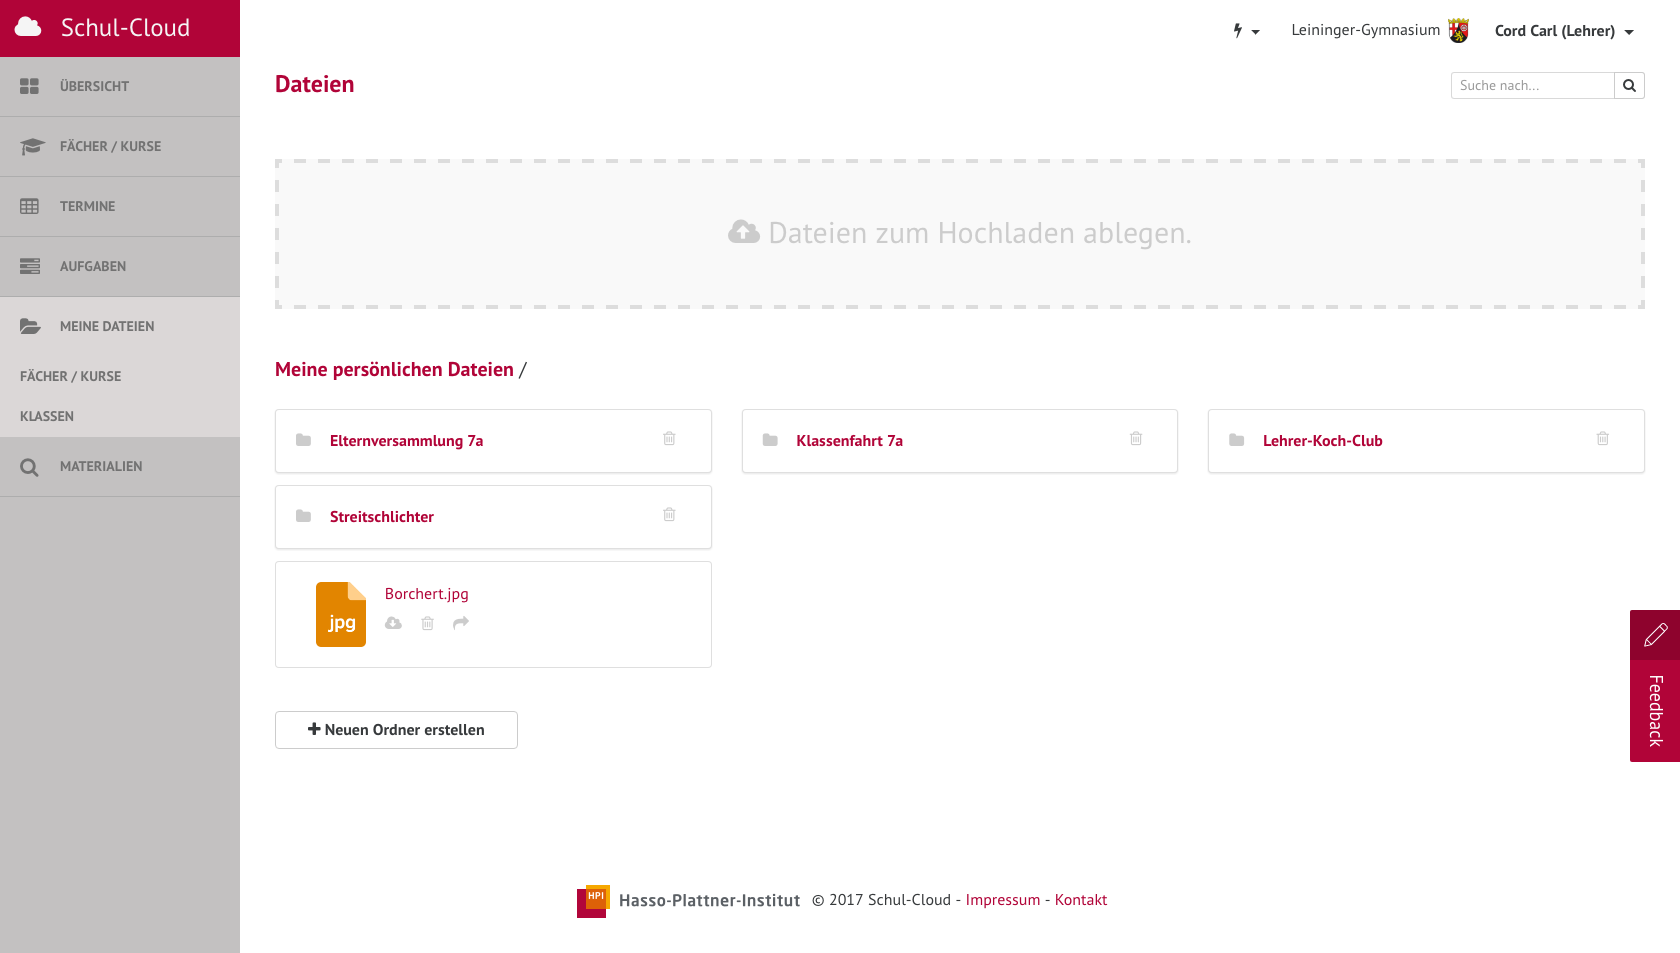
\includegraphics[width=1\linewidth]{images/screenMeineDateien}
	\caption[Caption for implementation]{Ansicht für die persönlichen Dateien}
	\label{fig:screenMeineDateien}
\end{figure}

Neben der normalen Dateiansicht für persönliche, Kurs - und Klassendateien hat man außerdem die Möglichkeit, als Lehrer Dateien direkt im Unterrichtskontext einzufügen. Dazu geht man auf einen Kurs, dann auf ein Thema, bearbeitet dieses Thema und fügt eine Text-Komponente hinzu. Hier wurde der eingebaute \textit{ckEditor} \footnote{ckEditor - \url{http://ckeditor.com/}} so überarbeitet, dass man entweder per Drag \& Drop eine Datei hineinschieben kann oder über die Bilderauswahl ein Bild aus dem Kurskontext auswählen kann (Abbildung \ref{fig:screenCkEditor}).

\begin{figure}[H]
	\centering
	\includegraphics[width=1\linewidth]{images/screenCkEditor}
	\caption[Caption for implementation]{Ansicht für das Hinzufügen einer Datei in den Unterrichtskontext}
	\label{fig:screenCkEditor}
\end{figure}

\subsubsection{Administration}
\subsubsection{File Sharing}

\clearpage
